\documentclass[
    11pt,
    aspectratio=169,
]{beamer}
\mode<beamer>{
\usetheme[hideothersubsections,
right,width=22mm]{Goettingen}
}
\usepackage[spanish]{babel} %Definir idioma español
\usepackage[utf8]{inputenc} %Codificacion utf-8
\usepackage{hyperref}
\title{Control continuo con aprendizaje por refuerzo profundo}
\author{Emmanuel Peto Gutiérrez}
\institute{IIMAS \\ UNAM}
\begin{document}

\begin{frame}<handout:0>
\titlepage
\end{frame}

\section{Aprendizaje por refuerzo}

% Frame
\begin{frame}
\frametitle{La interfaz agente-ambiente}

\begin{center}
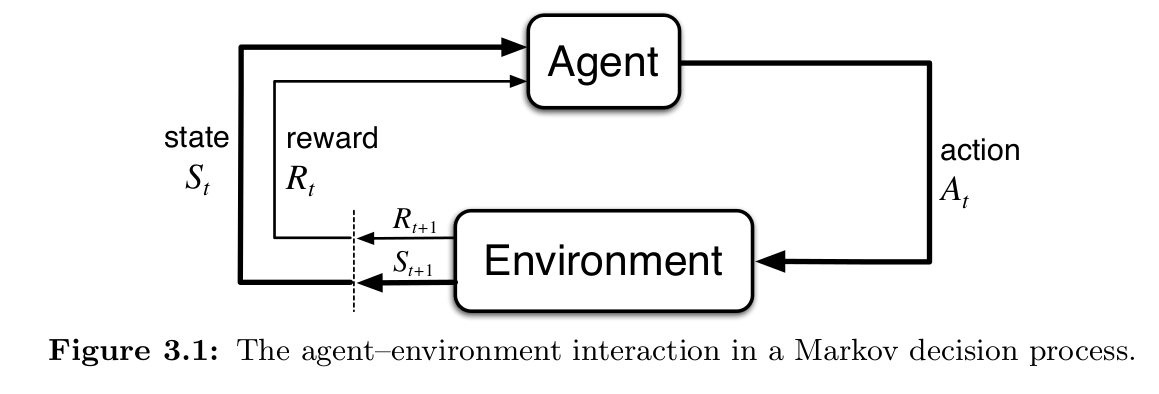
\includegraphics[scale=0.26]{Images/env_agent}
\end{center}

\end{frame}

% Frame
\begin{frame}
\frametitle{Conceptos}

\begin{itemize}
\item Política: $\pi (a|s)$ (probabilidad).
\item Retorno: $G_t = R_{t+1} + \gamma G_{t+1}$
\item Función de acción-valor: $Q_{\pi}(s,a)$ (retorno esperado).
\item Función de estado-valor: $v_{\pi}(s)$ (retorno esperado).
\item Política determinista: $\pi(a|s) = 1$ o $\mu(s) = a$.
\end{itemize}

\end{frame}

% Frame
\begin{frame}
\frametitle{Gradiente de política}

\begin{itemize}

\item Política parametrizada:

$\pi (a | s, \theta) = p(A_t = a | S_t=s, \theta_t = \theta)$

o si es determinista: $\mu (s | \theta)$

\item Medida de desempeño:

$J(\theta)$

\item Gradiente ascendente:

$\theta = \theta + \alpha \nabla J(\theta)$

\end{itemize}

\end{frame}

% Frame
\begin{frame}
\frametitle{Actor-critic}

Un método actor-crítico aprende las funciones de aproximación tanto para la política como para la función de valor.

\begin{itemize}
\item Actor: la función relacionada con la política ($\pi (a|s)$ o $\mu (s)$).
\item Crítico: la función relacionada con el valor ($q(s,a)$ o $v(s)$).
\end{itemize}

\begin{center}
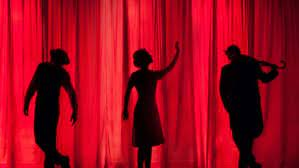
\includegraphics[scale=0.4]{Images/actores}
\end{center}

\end{frame}

\section{Antecedentes}

% Frame
\begin{frame}
\frametitle{El problema}

\textbf{Problema:} encontrar una política donde las variables acción ($a$) y (estado) $s$ son continuas, y probar resultados en problemas de control físico (como balancear un péndulo o manejar un carro).

\begin{center}
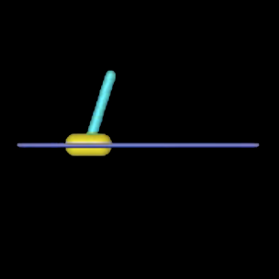
\includegraphics[scale=0.4]{Images/cartpole}
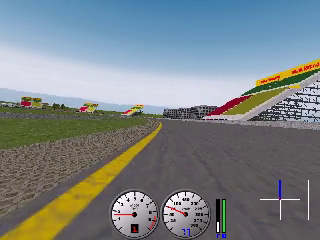
\includegraphics[scale=0.4]{Images/car_driving}
\end{center}

\end{frame}

% Frame
\begin{frame}
\frametitle{Solución}

Lo que se conoce hasta el momento de publicar el artículo (2016)

\begin{itemize}
\item Algoritmo Deep Q-Network (DQN)
\item Algoritmo Deterministic Policy Gradient (DPG)
\end{itemize}

\pause

\textbf{Solución:} combinar las ideas de los dos algoritmos para crear uno nuevo.

\end{frame}

% Frame
\begin{frame}
\frametitle{Pérdida para función Q}

Acción-valor dada una política determinista ($\mu : S \rightarrow A$)

$Q^{\mu} (s_t, a_t) = \mathbb{E} [r(s_t, a_t) + \gamma Q^{\mu} (s_{t+1}, \mu (s_{t+1}))]$

\pause

Se consideran aproximadores de funciones parametrizadas por $\theta$, con pérdida:

$L(\theta) = \mathbb{E} [(Q(s_t, a_t | \theta) - y_t)^2]$

donde

$y_t = r(s_t, a_t) + \gamma Q(s_{t+1},\mu (s_{t+1}) | \theta)$

\end{frame}

\section{El algoritmo}

% Frame
\begin{frame}
\frametitle{DDPG y aproximadores de funciones}

El nombre del algoritmo es \textit{Deep deterministic policy gradient} (DDPG). Usa redes neuronales para aproximar las funciones $\mu(s)$ y $Q(s,a)$.

\begin{itemize}
\item \textbf{Actor:} Red neuronal que mantiene una política parametrizada $\mu (s| \theta)$.
\item \textbf{Crítico:} Red neuronal que aproxima la función $Q(s,a| \theta)$. Se aprende usando la ecuación de Bellman como en Q-learning.
\end{itemize}

\pause

El algoritmo mantiene copias de las redes de $Q$ y $\mu$:

\begin{itemize}
\item $Q' (s,a | \theta^{Q'})$
\item $\mu' (s | \theta^{\mu '})$
\end{itemize}

\end{frame}

% Frame
\begin{frame}
\frametitle{La medida de desempeño}

\begin{itemize}
\item Medida:

$$ J(\mu) = \mathbb{E} [r(s, \mu (s | \theta))] $$

\item Gradiente:

$$\nabla_{\theta^{\mu}} J = \mathbb{E} [\nabla_a Q (s, a | \theta^Q) | _{s=s_t, a=\mu (s_t)} \nabla_{\theta_{\mu}} \mu (s | \theta^{\mu}) | _{s=s_t}]$$

\end{itemize}

\end{frame}

% Frame
\begin{frame}
\frametitle{Buffer de recuerdos}

Al usar una red neuronal como un aproximador de función se asume que los ejemplos son:

\begin{itemize}
\item Independientes
\item Identicamente distribuidos
\end{itemize}

Para ello se usa un \textit{buffer de recuerdos}, que es un espacio finito de memoria que almacena tuplas $(s_t, a_t, r_t, s_{t+1})$.

Nota: El algoritmo DQN también usa el buffer de recuerdos.

\end{frame}

% Frame
\begin{frame}
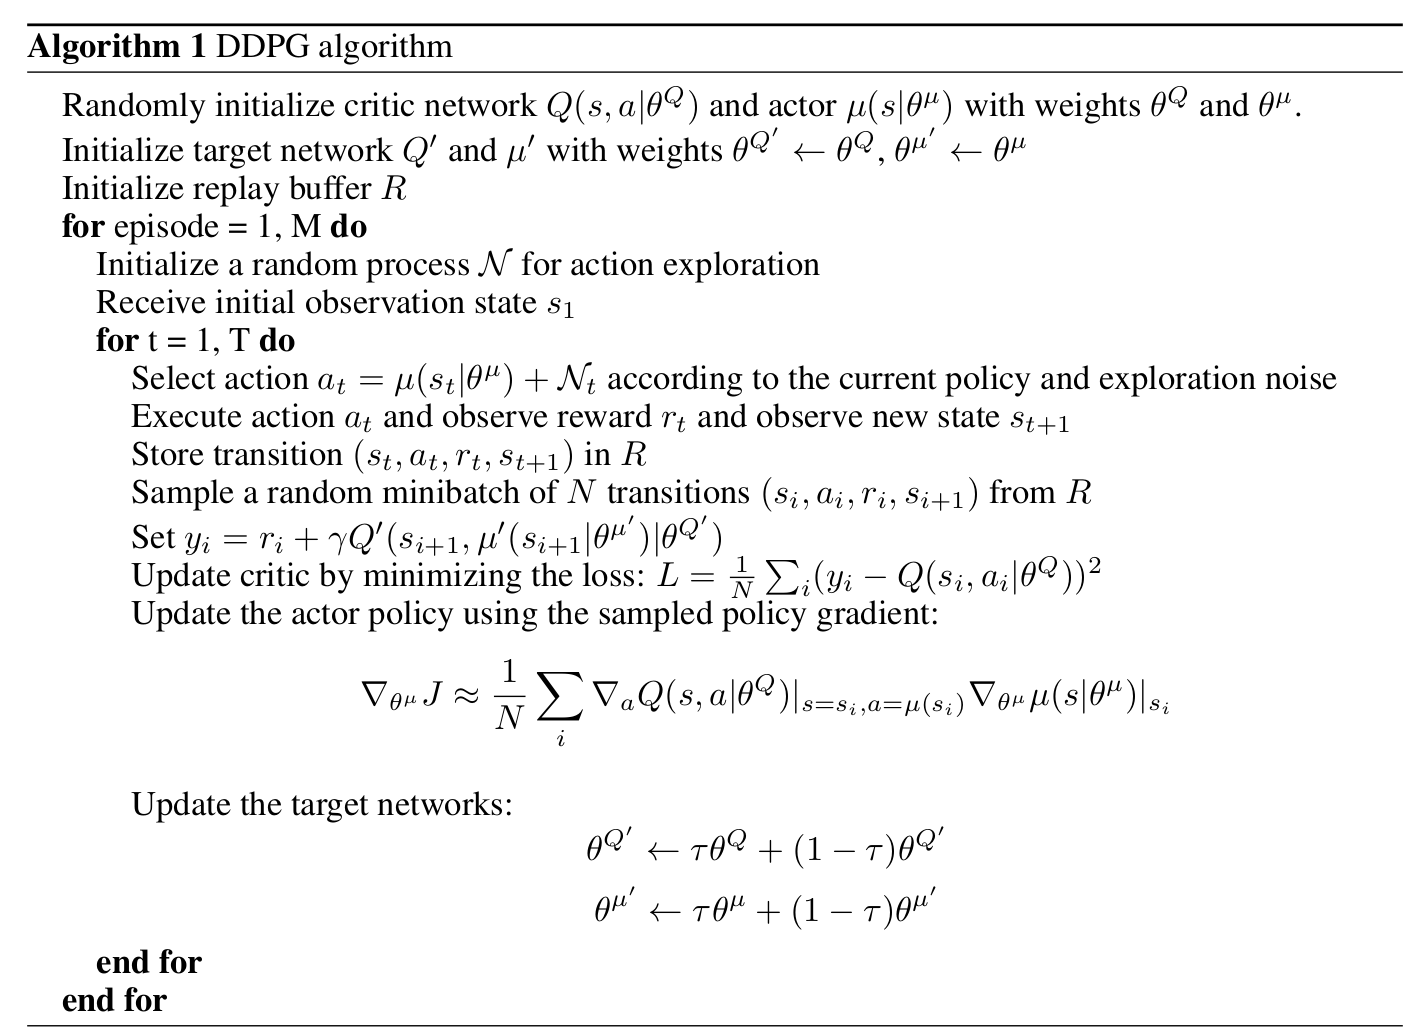
\includegraphics[scale=0.2]{Images/ddpg}
\end{frame}

\section{Resultados}

% Frame
\begin{frame}
\frametitle{Experimentos}

Para la simulación de ambientes se utilizó MuJoCo. Para la representación de estados se usó primero una descripción de baja dimensión (como la posición y el ángulo) y luego imágenes de $64 \times 64$.

Se realizó el experimento con 4 variantes del algoritmo.

\begin{itemize}
\item DPG con normalización por lotes.
\item Con red objetivo.
\item Con red objetivo y normalización por lotes.
\item Con red objetivo usando solo pixeles.
\end{itemize}

\end{frame}

% Frame
\begin{frame}
\frametitle{Retorno}

Se puede observar la recompensa normalizada (eje $y$) después de millones de pasos (eje $x$) en algunos ambientes. El color de la gráfica representa la variante del algoritmo: normalización por lotes (gris claro), red objetivo (gris oscuro), red objetivo y normalización por lotes (verde), red objetivo usando solo pixeles (azul).

\begin{center}
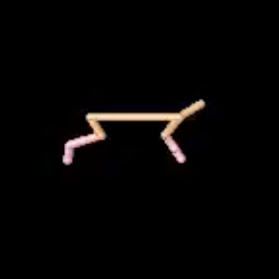
\includegraphics[scale=0.2]{Images/cheetah}
\hspace{5mm}
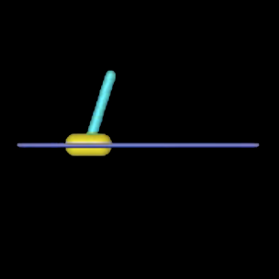
\includegraphics[scale=0.2]{Images/cartpole}

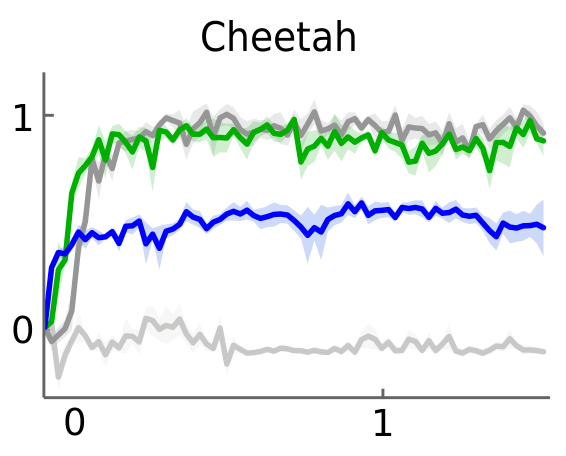
\includegraphics[scale=0.2]{Images/cheetah_grafica}
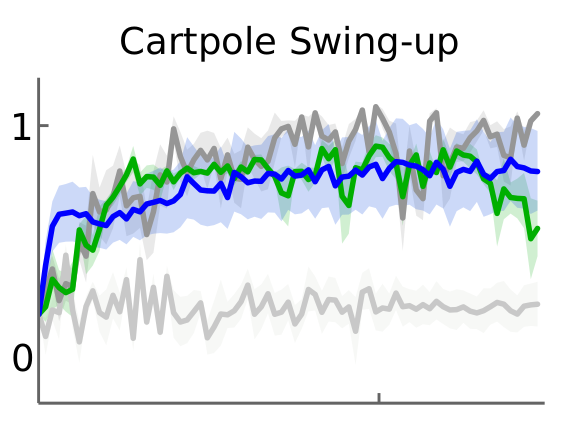
\includegraphics[scale=0.2]{Images/cartpole_grafica}
\end{center}

\end{frame}

\section{Conclusiones}

%Frame
\begin{frame}
\frametitle{Conclusiones}

\begin{itemize}
\item La combinación de los avances en RL y DeepL resultan en algoritmos que resuelven problemas a lo largo de una variedad de dominios con espacios de acción continuos.
\item Los experimentos realizados usaron menos pasos que los usados por DQN para encontrar soluciones en el dominio de Atari.
\item DDPG requiere un gran número de episodios de entrenamiento para encontrar soluciones.
\end{itemize}

\end{frame}

\section{Apéndices}

% Frame
\begin{frame}

\begin{center}
{\huge Apéndices}
\end{center}

\end{frame}

% Frame
\begin{frame}
\frametitle{Paper}

\begin{center}
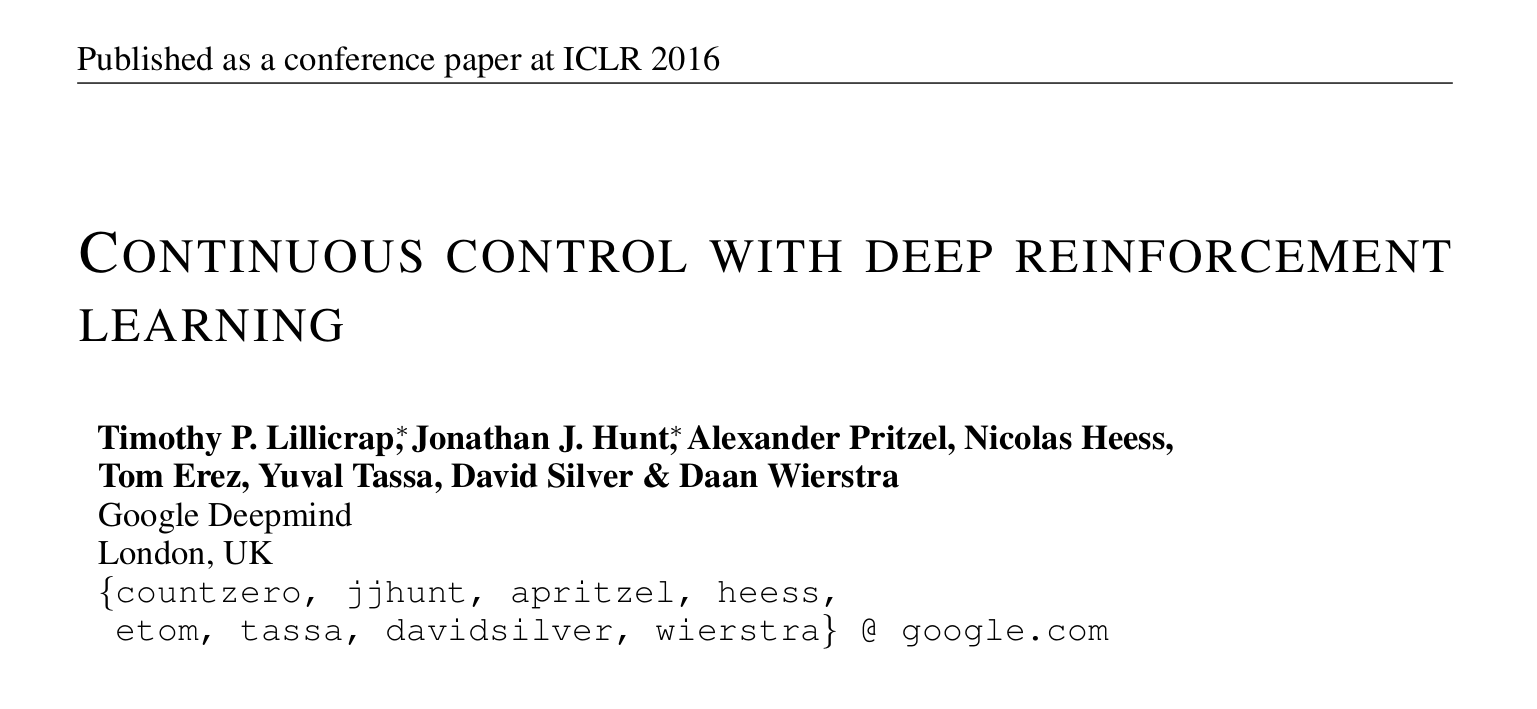
\includegraphics[scale=0.2]{Images/continuous_control}
\end{center}

\end{frame}

% Frame
\begin{frame}
\frametitle{MuJoCo}

El enlace a los videos que está en el paper te lleva a videos privados. Sin embargo, se pueden observar algunos ambientes de MuJoCo en los siguientes videos:

\begin{itemize}
\item Cheetah: \url{https://youtu.be/emuPEFYkIYo?si=eKOCZHP9BBa8eFo7}
\item Cartpole: \url{https://youtu.be/fXbqDDaJDvg?si=aeEZCLdTRpVcFWRr}
\end{itemize}

\end{frame}

% Frame
\begin{frame}
\frametitle{Q-learning}

\begin{center}
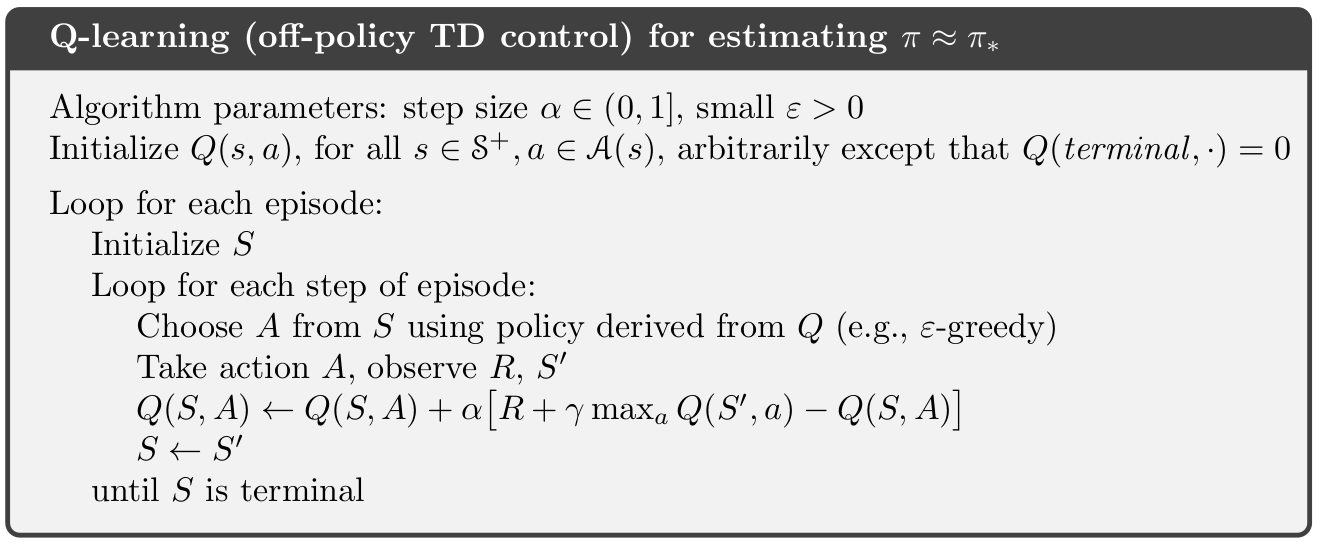
\includegraphics[scale=0.25]{Images/q_learning}
\end{center}

\end{frame}

% Frame
\begin{frame}
\frametitle{DQN}

\begin{center}
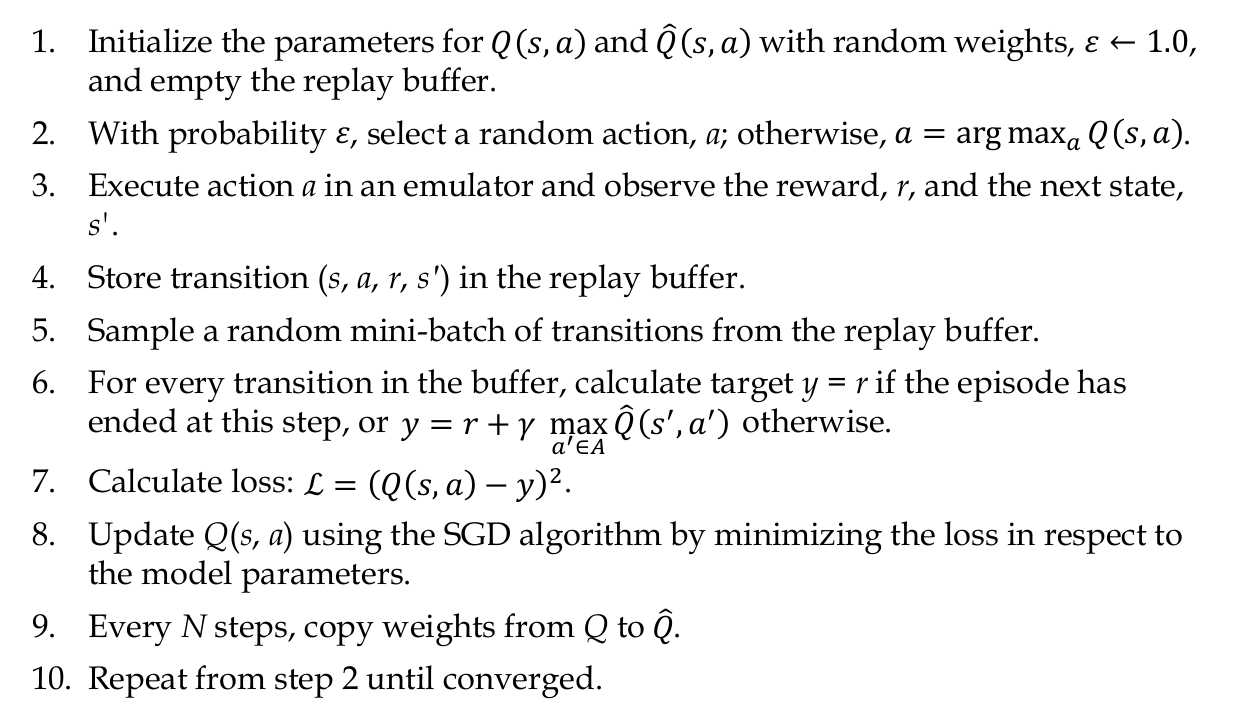
\includegraphics[scale=0.25]{Images/dqn}
\end{center}

\end{frame}

% Frame
\begin{frame}
\frametitle{Hiperparámetros}

\begin{itemize}
\item Aprendizaje de la red: Adam
\item Tasa de aprendizaje del actor: $10^{-4}$
\item Tasa de aprendizaje del crítico: $10^{-3}$
\item Factor de descuento ($\gamma$): 0.99
\item $\tau$: 0.001
\end{itemize}

\end{frame}

% Frame
\begin{frame}
\frametitle{Arquitectura de red}

\begin{itemize}
\item Función de activación en capas ocultas: rectified non-linear.
\item Función de activación en última capa: tanh.
\item Para ambientes de baja dimensión: 2 capas ocultas con 400 y 300 neuronas respectivamente.
\item Para ambientes de pixeles: 3 capas convolucionales con 32 filtros, seguido de dos capas densas de 200 neuronas.
\end{itemize}

\end{frame}

\end{document}

